\documentclass[a4paper,14pt]{article}

\usepackage[14pt]{extsizes}
\usepackage{cmap}					% поиск в PDF
\usepackage{mathtext} 				% русские буквы в формулах
\usepackage[T2A]{fontenc}			% кодировка
\usepackage[utf8]{inputenc}			% кодировка исходного текста
\usepackage[english,russian]{babel}	% локализация и переносы
\usepackage{graphicx}
\usepackage{geometry}
\usepackage{amsmath}
\usepackage{amssymb}
\usepackage[table]{xcolor}
\setlength\extrarowheight{2pt}


\geometry{verbose, a4paper, tmargin=2cm, bmargin=2cm, lmargin=2cm, rmargin=2cm}
\author{Vysotsky Maxim}
\title{Отчёт}
\date{2025}

\begin{document}
	\begin{titlepage}
		\begin{center}
			{Министерство науки и высшего образования Российской Федерации
				НОВОСИБИРСКИЙ НАЦИОНАЛЬНЫЙ ИССЛЕДОВАТЕЛЬСКИЙ
				ГОСУДАРСТВЕННЫЙ УНИВЕРСИТЕТ (НГУ)}
		\end{center}
		\begin{center}
			{Физический факультет}
		\end{center}
		\begin{center}
			{Кафедра общей физики}
		\end{center}
		
		
		\vspace{7cm}
		{
			\begin{center}
				{\bf Лабораторная работа №2.4}\\
			Наблюдение фазовых переходов «жидкость – газ» и определение
критической температуры Фреона-13
			\end{center}
		}
		\vspace{2cm}
		\begin{flushright}
			{Руководитель:\\ Ассистент\\
				Художитков В. Э.\\
                Старший преподаватель \\
                Кравцова А. Ю.\\
				Работу выполнил:\\
				Высоцкий М. Ю.\\
				\vspace{0.2cm}
				гр. 24301}
		\end{flushright}
		\vspace{3cm}
		\begin{center}
			Новосибирск, 2025
		\end{center}
	\end{titlepage}


\section{Теоретическое введение}

\hspace{\parindent}\textbf{Цель работы:} знакомство с фазовыми переходами, определение
линии равновесия «жидкость – пар» в \textbf{Tv}-координатах, наблюдение
критического состояния вещества.

\textbf{Оборудование:} ампулы с исследуемым веществом, термостат,
ртутный термометр.

\textbf{Фазовый переход} – это скачкообразный переход вещества из
одной фазы в другую при непрерывном изменении
внешних условий – температуры, давления, магнитных и
электрических полей и др. Фазовые переходы – широко
распространенное в природе явление. К ним относятся испарение и
конденсация (переход «жидкость – газ»), плавление и затвердевание
(переход «твердое тело – жидкость»), сублимация и конденсация в
твердую фазу (переход «твердое тело – газ»), а также некоторые
структурные переходы в твердых телах.

\textbf{Критическая точка} – точка температуры и давления на фазовой диаграмме, где жидкая и газообразная фазы вещества сливаются в одну фазу. В данной точке фазы теряют качественные различия.

\textbf{Метастабильное состояние} - состояние системы, при котором его стабильность хорошо сохраняется при малых возмущениях. 

\textbf{Уравнение Менделеева-Клапейрона} (уравнение состояние газа):
$$
    Pv\mu-RT=0
$$




Ниже приведена схема установки.

\begin{figure}[h]
    \centering
    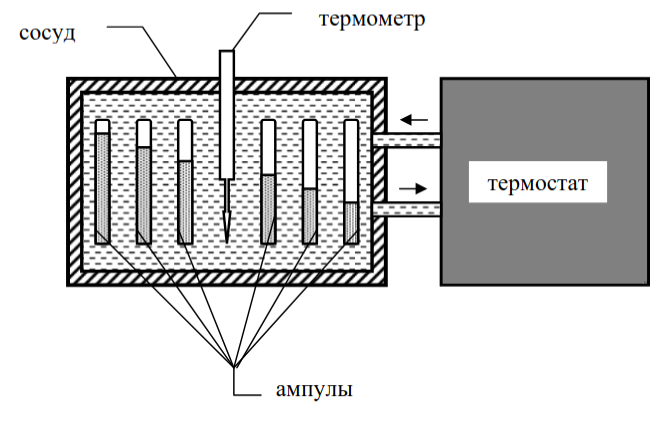
\includegraphics[scale=0.8]{scheme.png}
    \caption{Схема установки.}
\end{figure}

\clearpage

\begin{figure}[h]
    \centering
    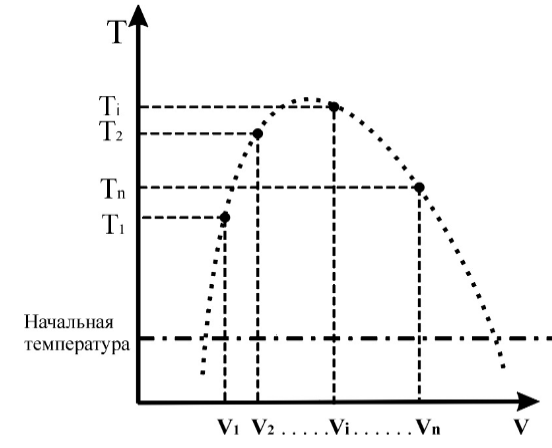
\includegraphics[scale=0.8]{TV.png}
    \caption{Определение кривой равновесия
«жидкость – пар» в Tv-плоскости.}
\end{figure}


\subsection{Ход эксперимента}

Ниже приведены данные эксперимента.


\begin{table}[!ht]
    \centering
    \begin{tabular}{|l|l|l|l|l|l|}
    \hline
        № & Исчезн. , С & Исчезн. , К & Появл. , С & Появл. , К & Уд. Объем, $см^3/г$ \\ \hline
        1 & 25 & 298 & 25 & 298 & 0,9 \\ \hline
        2 & 27,75 & 300,75 & 28,65 & 301,65 & 1,328 \\ \hline
        3 & 28,55 & 301,55 & 28,95 & 301,95 & 1,364 \\ \hline
        4 & 29,25 & 302,25 & 29,15 & 302,15 & 1,59 \\ \hline
        5 & 28 & 301 & 29,35 & 302,35 & 2 \\ \hline
        6 & 27,45 & 300,45 & 26,35 & 299,35 & 2,45 \\ \hline
    \end{tabular}
    \caption{Данные эксперимента.}
\end{table}
\clearpage
Далее по данным был построен график с аппроксимацией.

\begin{figure}[h]
    \centering
    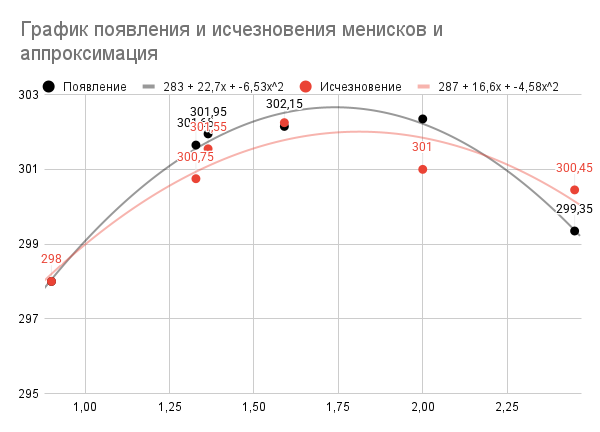
\includegraphics[scale=0.7]{exp.png}
    \caption{Появление и исчезновение менисков.}
\end{figure}



Из аппроксимации (полиномиальной) получены следующие данные:
\begin{table}[!h]
    \centering
    \begin{tabular}{|l|l|l|l|l|}
    \hline
         & $T_{кр}$, К, & К $T_{кр}$, С & $v$, $см^3/г$ & $\rho_{кр}$, $кг/м^3$ \\ \hline
        Нагрев & 302,73 & 29,73 & 1,81 & 552,49 \\ \hline
        Охлад & 302,04 & 29,04 & 1,74 & 574,71 \\ \hline
    \end{tabular}
    \caption{Критическкие температуры и удельные объемы.}
\end{table}

\section{Вывод}

Были найдены критические температуры для охлаждения и нагрева Фреона-13, а также их критические удельные объёмы.

$$Т_{кр(охл.)} = 29,04^\circ C$$
$$Т_{кр(нагр.)} = 29,73^\circ C$$
$$v_{кр(охл.)} = 1,74 см^3/г$$
$$v_{кр(нагр.)} = 1,81 см^3/г$$

\end{document}
